% ------------------------------------------------------------------------ %
% !TEX encoding = UTF-8
% !TEX TS-program = pdflatex
% !TEX root = ../Project.tex
% !TEX spellcheck = en-EN
% ------------------------------------------------------------------------ %
%
% ------------------------------------------------------------------------ %
% 	CHAPTER TITLE
% ------------------------------------------------------------------------ %
%
\chapter{UML Models}
%
\label{cap:umlmodels}
In the following pages are present some models that describe the system and its functionalities.
%
% ------------------------------------------------------------------------ %
%
\section{Use cases}
\begin{center}
\makebox[\textwidth][c]{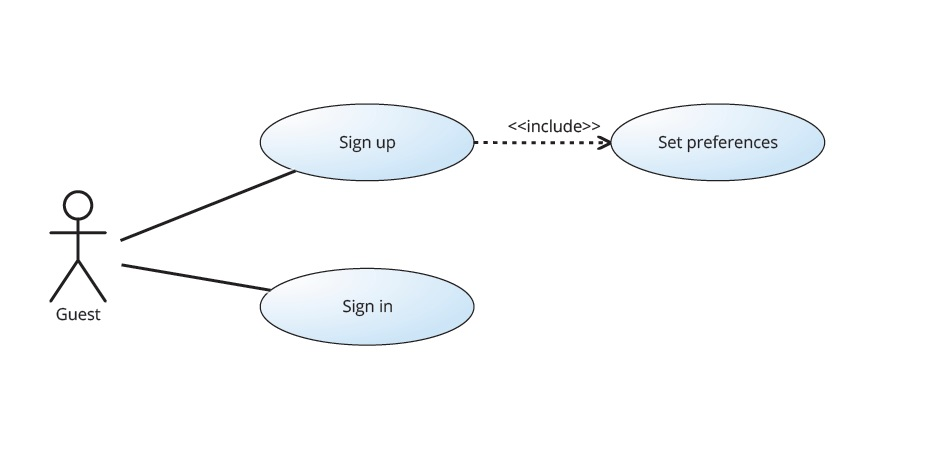
\includegraphics[width=1.1\textwidth]{MainMatter/images/usecases/guest}}
\captionof{figure}{Guest's use case diagram}
\makebox[\textwidth][c]{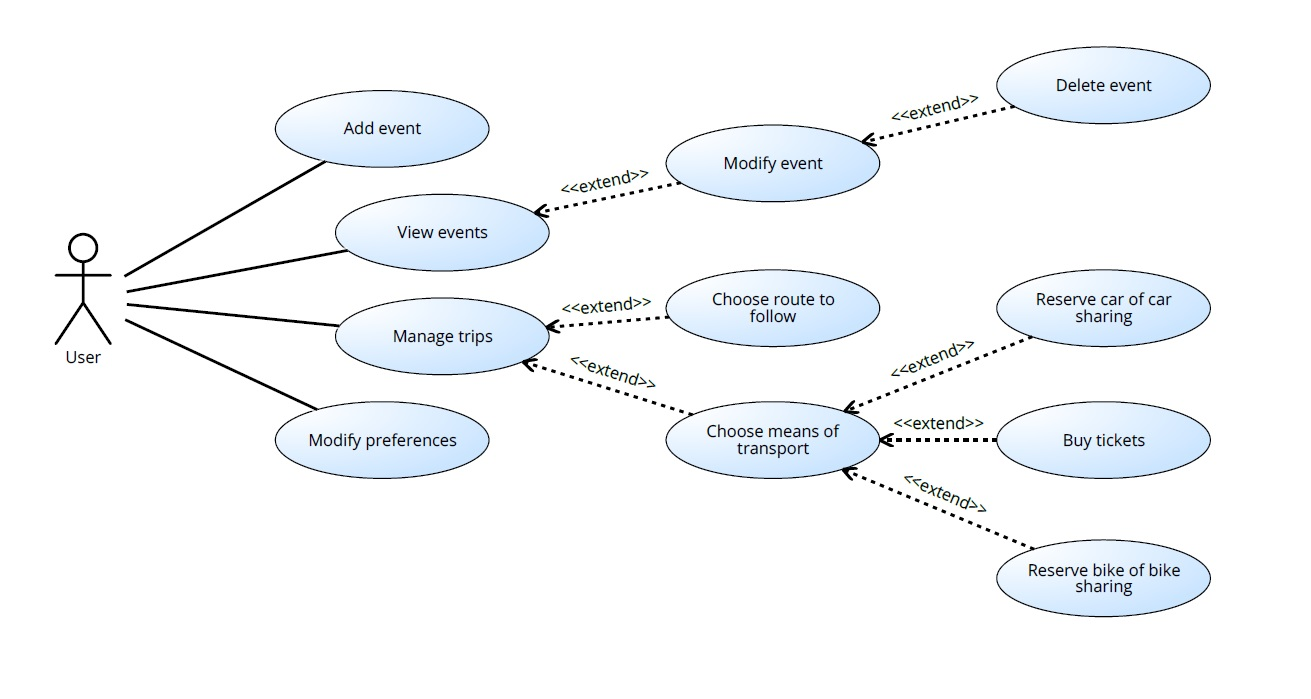
\includegraphics[width=1.4\textwidth]{MainMatter/images/usecases/user}}
\captionof{figure}{User's use case diagram}
\end{center}
\pagebreak
%
\begin{landscape}
\section{Class diagram}
\begin{center}
\thispagestyle{empty}
\makebox[\textwidth][c]{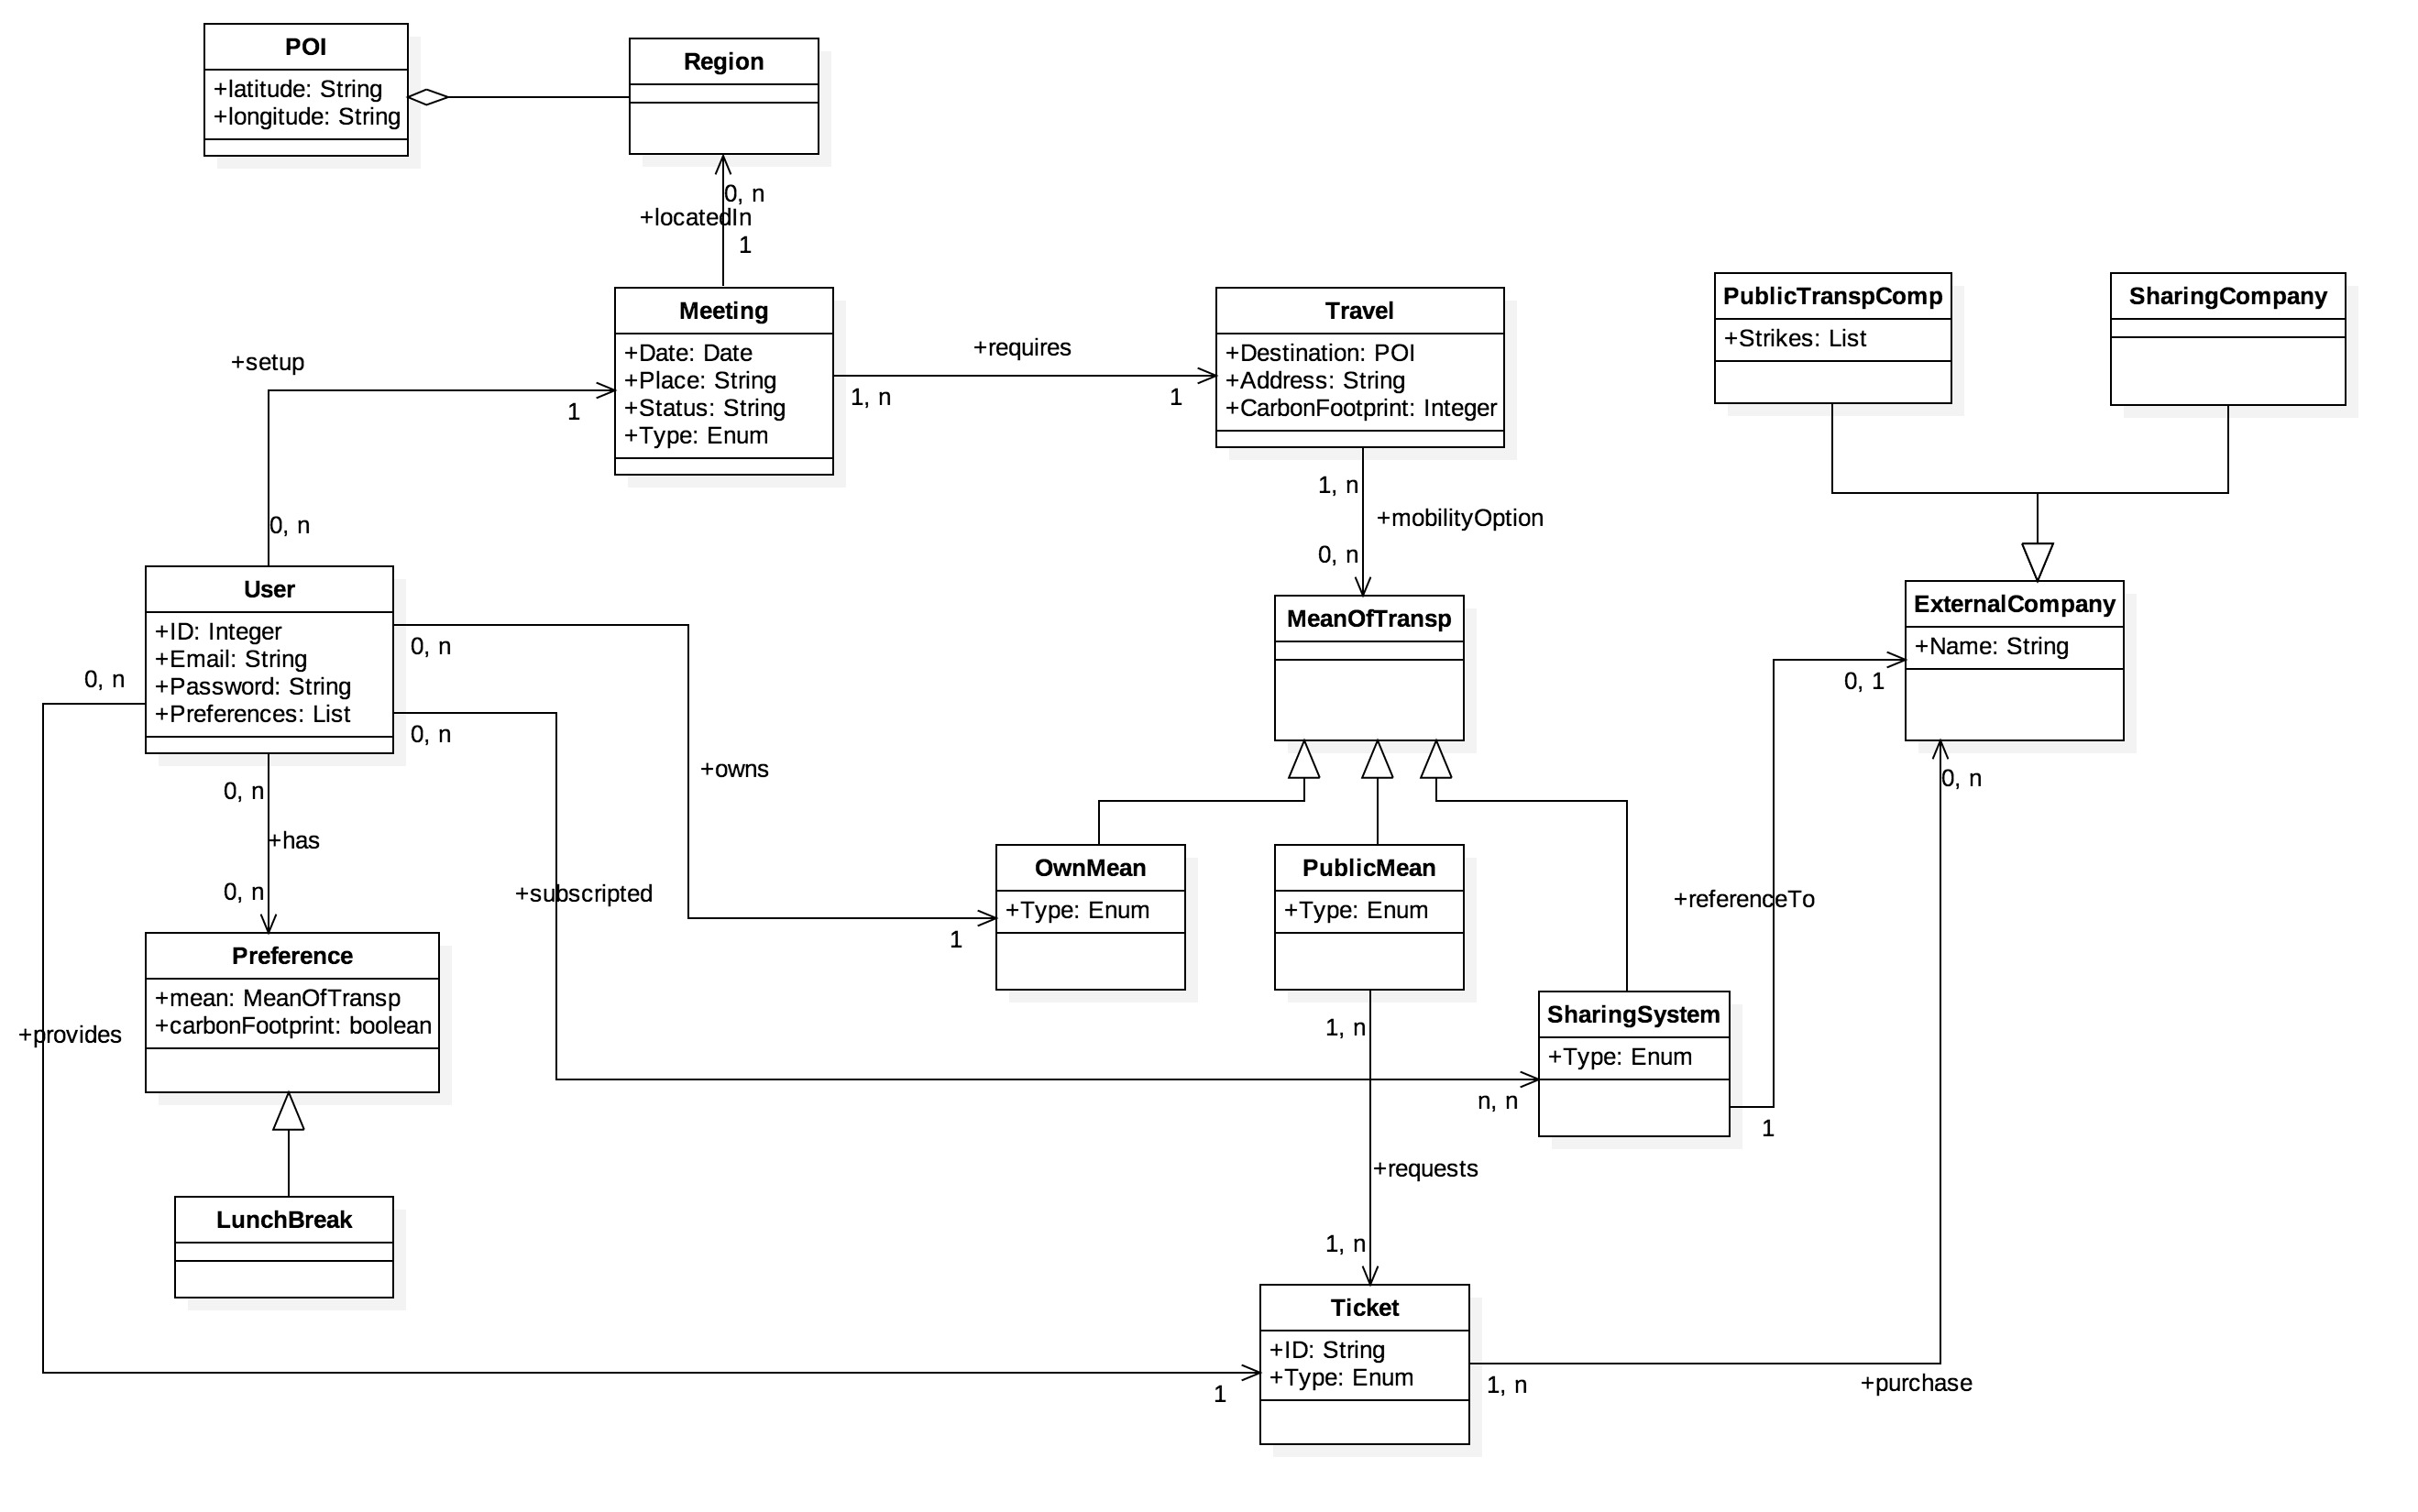
\includegraphics[width=1.3\textwidth]{MainMatter/images/uml/uml}}
\captionof{figure}{Class diagram of the application}
\end{center}
\end{landscape}
%

\section{Use case description}
In this section some use cases will be described. These use cases can be
derived from the scenarios and the use case diagram.
%
\begin{center}
\def\arraystretch{1.2}
  \begin{tabular}{ | l | p{0.65\textwidth} | }
    \hline
    Name & Sign up \\ \hline
    Primary Actor & Guest \\ \hline
    Preconditions & The guest wants to register to “Travlendar+” \\ \hline
    Postconditions & Guest's informations are stored in the “Travlendar+” server and locally on the device. The Guest can sign in to use the application, becoming a user \\ \hline
    Flow of events  & 1.	The guest opens the application for the first time \\
					& 2.	The system shows the Login screen to the guest \\
					& 3.	The Guest clicks on “Sign Up” \\
					& 4.	The System shows to the Guest the Registration page \\
					& 5.	The guest inserts his personal details (name, surname, …) and his trip preferences (important addresses, owned car, season ticket, …) \\
					& 6.	The guest reads and accepts the user agreement \\
					& 7.	The guest taps on “Confirm” \\
					& 8.	The system check the correctness of the data and sends an email and a sms with a verification link \\
					& 9.	The guest confirms his registration clicking on one of the verification links \\
					& 10.	The guest is now registered and becomes a User of “Travlendar+” \\
					& 11.	The system shows to the user the Main screen (Calendar) of the application \\ \hline    
    Exceptions  & 1.	One or more fields of the Registration page are not well formed \\
				& 2.	Username is already in use \\
				& 3.	Email is already in use \\
				& 4.	The verification link is expired (after 24 hours)\\ \hline
  \end{tabular}
\captionof{table}{Use case for sign up}
\end{center}

\begin{center}
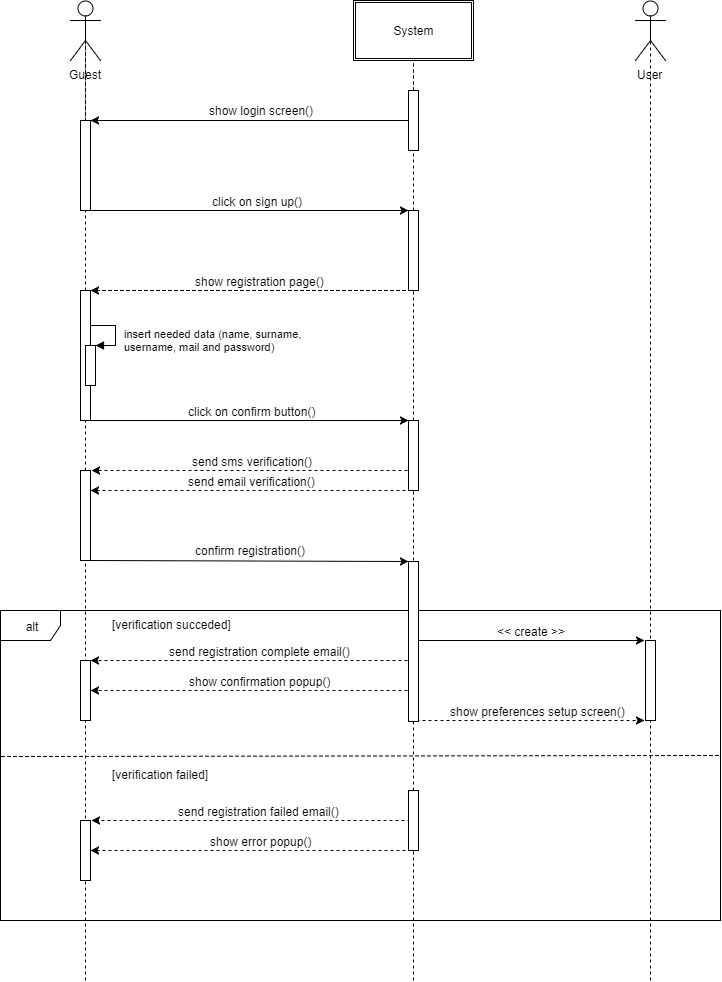
\includegraphics[scale=0.55]{MainMatter/images/sequencediagrams/signup}
\captionof{figure}{Sequence diagram of sign up use case}
\end{center}

\begin{center}
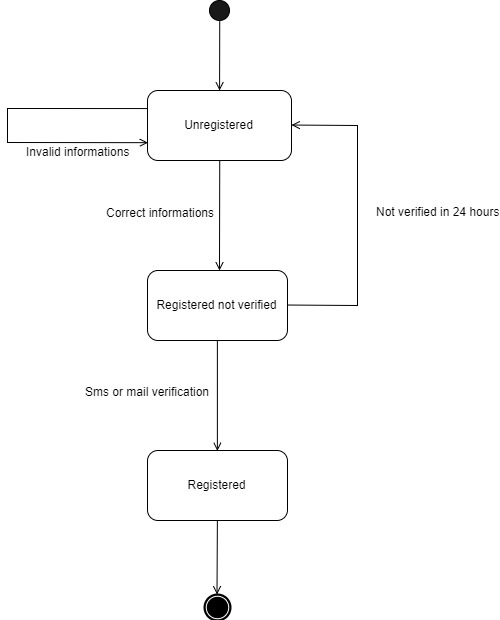
\includegraphics[scale=0.8]{MainMatter/images/statecharts/signup}
\captionof{figure}{Statechart of sign up process}
\end{center}

\begin{center}
\def\arraystretch{1.25}
  \begin{tabular}{ | l | p{0.65\textwidth} | }
    \hline
    Name & Sign in \\ \hline
    Primary Actor & Guest \\ \hline
    Preconditions & The guest wants to sign in to use “Travlendar+”. He is actually an user of the application because he has a valid account for it \\ \hline
    Postconditions & The guest is now logged into the system becoming an user \\ \hline
    Flow of events  & 1.	The guest opens the application \\
					& 2.	The system shows to the guest the Login screen \\
					& 3.	The guest inserts account credentials (username and password) \\
					& 4.	The guest taps on “Sign In” \\
					& 5.	The system checks if the credentials  are present in the database \\
					& 6.	The guest is now logged and becomes an user \\
					& 7.	The system shows to the user the Main screen of the application \\ \hline    
    Exceptions  & 1.	One or more fields of the Login page are not well formed \\
    			& 2.	Username is not present in the database \\
				& 3.	The password associated to the username is incorrect \\ \hline
  \end{tabular}
\captionof{table}{Use case for sign in}
\end{center}

\begin{center}
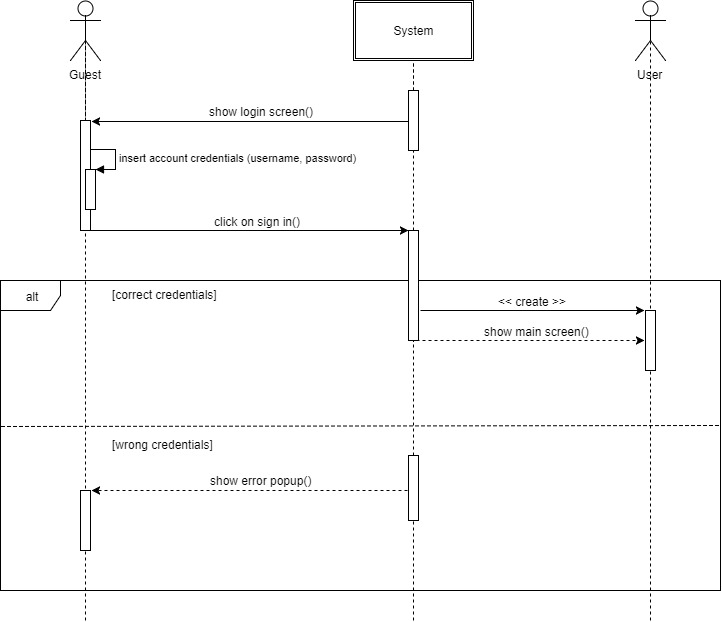
\includegraphics[scale=0.55]{MainMatter/images/sequencediagrams/signin}
\captionof{figure}{Sequence diagram of sign in use case}
\end{center}


\begin{center}
\def\arraystretch{1.25}
  \begin{tabular}{ | l | p{0.65\textwidth} | }
    \hline
    Name & Add event to calendar \\ \hline
    Primary Actor & User \\ \hline
    Preconditions & The user wants to add an event to the calendar of his application. He is already logged in into the service and the system is showing the calendar \\ \hline
    Postconditions & The event is added to the calendar and stored in the database, the system computes the round trip from the location of the event and shows again the calendar to the user \\ \hline
    Flow of events  & 1.	The user taps on “Add Event” (the red button with a white cross) \\
					& 2.	The system shows the Add Event screen \\
					& 3.	The user inserts the details in the requested fields \\
					& 4.	The user clicks on “Confirm” \\
					& 5.	The system adds the event to the calendar and shows the updated Main screen to the user \\
 \hline    
    Exceptions  & 1.	The event overlaps with another one \\
				& 2.	The event overlaps with user’s lunch \\
				& 3.	One or more field are not well formed \\
				& 4.	The user cannot arrive in time for the event \\
 \hline
  \end{tabular}
\captionof{table}{Use case for add event}
\end{center}

\begin{center}
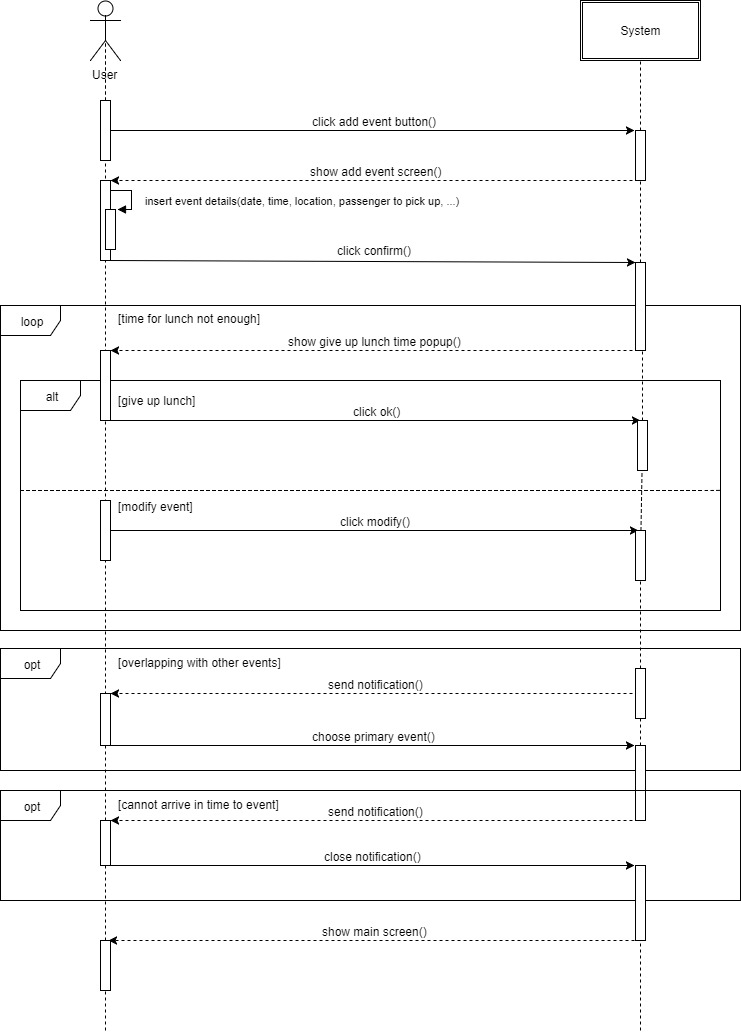
\includegraphics[scale=0.55]{MainMatter/images/sequencediagrams/add}
\captionof{figure}{Sequence diagram of add event use case}
\end{center}

\begin{center}
\def\arraystretch{1.25}
  \begin{tabular}{ | l | p{0.65\textwidth} | }
    \hline
    Name & Delete event from calendar \\ \hline
    Primary Actor & User \\ \hline
    Preconditions & The user wants to delete an event from the calendar of his application. He is already logged in into the service and the system is showing the calendar \\ \hline
    Postconditions & The event is deleted from the calendar and from the database, the system shows again the calendar to the user \\ \hline
    Flow of events  & 1.	The user selects the event he wants to delete \\
					& 2.	The system shows the Event Details screen \\
					& 3.	The user taps on “Modify Event” \\
					& 4.	The system shows Event Edit screen \\
					& 5.	The user clicks on “Delete Event” \\
					& 6.	The system deletes the event from the calendar and from the database, and shows the updated calendar to the user \\
 \hline    
    Exceptions  & 1.	The event overlaps with at least other two events and it is primary \\
 \hline
  \end{tabular}
\captionof{table}{Use case for delete event}
\end{center}

\begin{center}
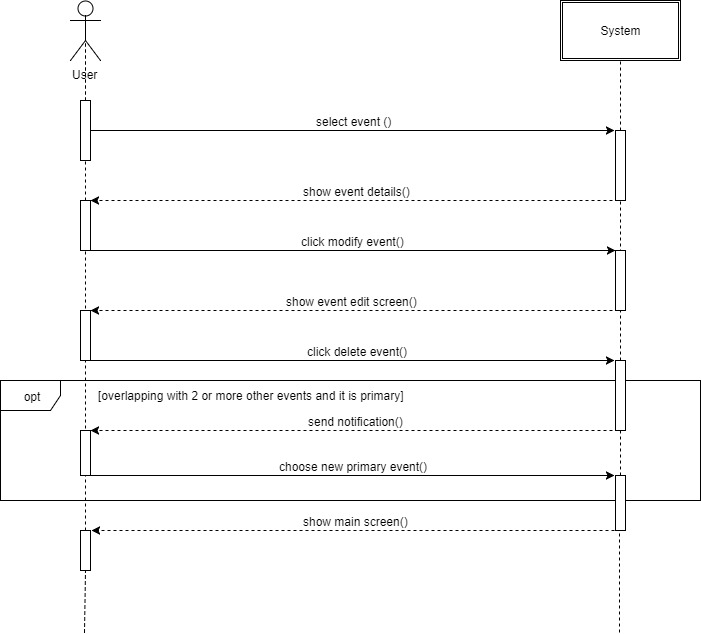
\includegraphics[scale=0.55]{MainMatter/images/sequencediagrams/delete}
\captionof{figure}{Sequence diagram of delete event use case}
\end{center}

\begin{center}
\def\arraystretch{1.25}
  \begin{tabular}{ | l | p{0.65\textwidth} | }
    \hline
    Name & Arrange trip \\ \hline
    Primary Actor & User \\ \hline
    Preconditions & The user wants to buy the tickets to take a trip. He is already logged in into the service and the system is showing the calendar \\ \hline
    Postconditions & The user receives the tickets \\ \hline
    Flow of events  & 1.	The user clicks on “Trips” (the button with the airplane) \\
					& 2.	The system shows the Trips screen \\
					& 3.	The user chooses the event he wants to buy the tickets for \\
					& 4.	The system shows the Trip details screen \\
					& 5.	The user clicks “Buy Now” \\
					& 6.	The system opens a link to buy the ticket and shows the checkout page to the user for every ticket purchasable online \\
					& 7.	The user pays and confirms for all the tickets \\
					& 8.	The system calls the External services that send the tickets to the user  \\
					& 9.	The user communicate to the system that the tickets are bought \\
 \hline    
 	Alternative flow    & 1.	The same operations as above until point 5 \\
						& 2.	The system calls the External services applications that show the checkout screen to the user, for every ticket only purchasable through the proprietary application \\
						& 3.	The user pays and confirms for all the tickets \\
						& 4.	The External services applications send the tickets to user \\
						& 5.	The user communicate to the system that the tickets are bought \\
 \hline
    Exceptions  & 1.	One or more payment failed \\
				& 2.	The user doesn’t confirm payment for one or more tickets \\
 \hline
  \end{tabular}
\captionof{table}{Use case for arrange trip}
\end{center}

\begin{center}
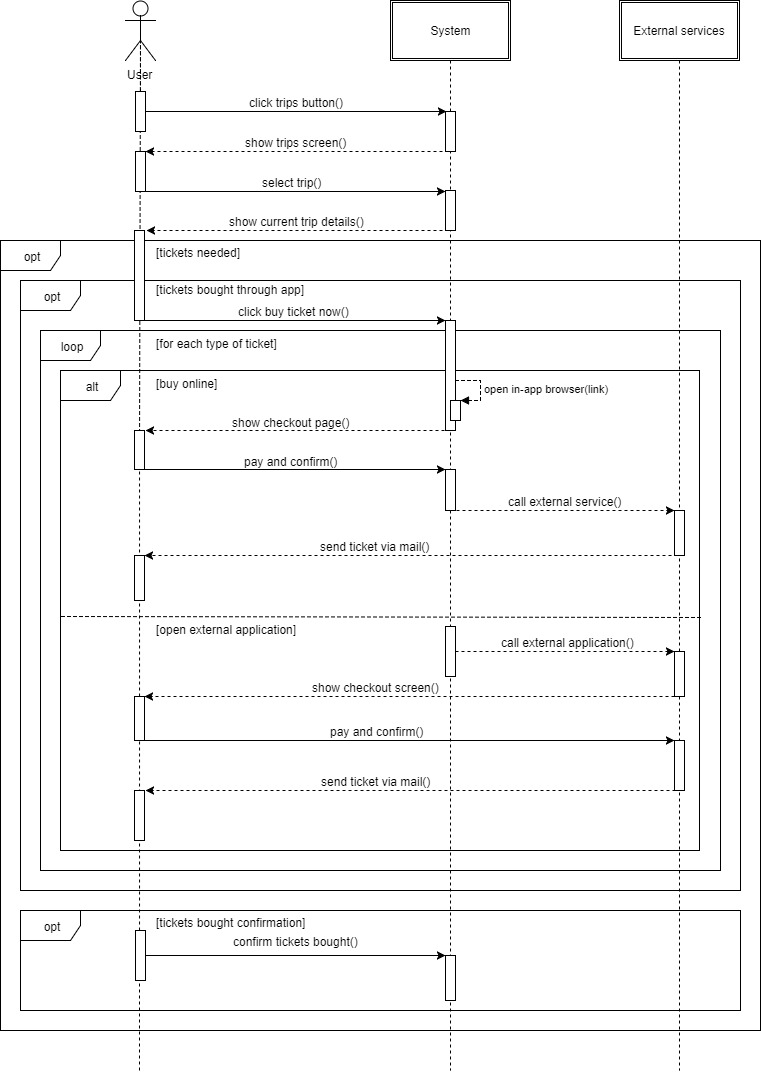
\includegraphics[scale=0.519]{MainMatter/images/sequencediagrams/arrange}
\captionof{figure}{Sequence diagram of arrange trip}
\end{center}

\begin{center}
\def\arraystretch{1.162}
  \begin{tabular}{ | l | p{0.65\textwidth} | }
    \hline
    Name & Manage trip options (customized trip) \\ \hline
    Primary Actor & User \\ \hline
    Preconditions & The user wants to change the modality of one of his trips, choosing to customize it and changing the preferred means of transport. He is already logged in into the service and the system is showing the calendar \\ \hline
    Postconditions & The trip is saved and changed as the user prefers \\ \hline
    Flow of events  & 1.	The user clicks on “Trips” (the button with the airplane) \\
					& 2.	The system shows the Trips screen \\
					& 3.	The user chooses the event he wants to modify \\
					& 4.	The system shows the Trip details screen \\
					& 5.	The user clicks “Modify” \\
					& 6.	The system shows Suggested Trip Choices screen \\
					& 7.	The user select “Customized” \\
					& 8.	The system calculates all available trip options and shows them to the user in the Trip Options screen \\
					& 9.	The user chooses new preferred means of transport \\
					& 10.	The system recalculate all the trip options with the User selection and show them to the user in the Trip Options screen \\
					& 11.	The user chooses his preferred trip option \\
					& 12.	The system shows the Trip details screen \\
					& 13.	The user selects back (the arrow icon) \\
					& 14.	The system shows the Main screen to the user
\\
 \hline
    Exceptions  & 1.	The user chooses to go only by foot but the distance to walk is wider than the one set in the preferences \\
				& 2.	The user chooses to go only by bike, but the time is not inside the interval chosen in the preferences
 \\
 \hline
  \end{tabular}
\captionof{table}{Use case for manage trip options, in the case that the user chooses to customize the trip}
\end{center}

\begin{center}
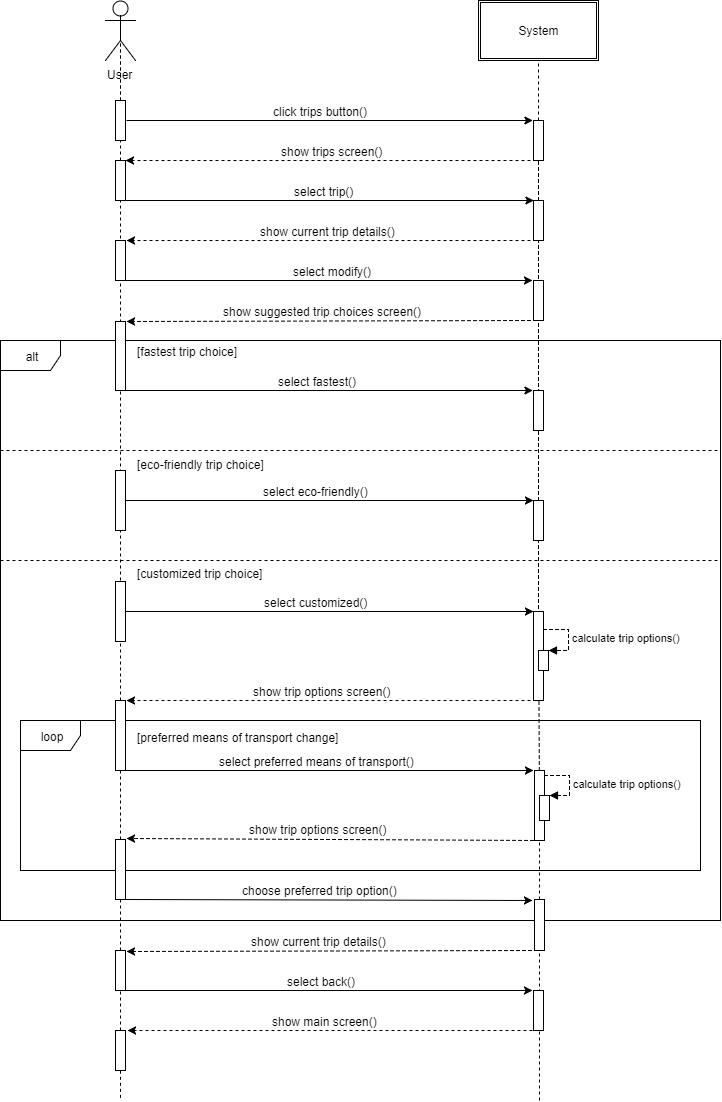
\includegraphics[scale=0.516]{MainMatter/images/sequencediagrams/managetrip}
\captionof{figure}{Sequence diagram of manage trip options}
\end{center}

\begin{center}
\def\arraystretch{1.25}
  \begin{tabular}{ | l | p{0.65\textwidth} | }
    \hline
    Name & Reserve a sharing means of transport \\ \hline
    Primary Actor & User \\ \hline
    Preconditions & The user wants to reserve a sharing means of transport. He is already logged in into the service and the system is showing the calendar \\ \hline
    Postconditions & The user has reserved the means of transport chosen and receives a confirmation via mail \\ \hline
    Flow of events  & 1.	The user clicks on “Trips” (the button with the airplane) \\
					& 2.	The system shows the Trips screen \\
					& 3.	The user chooses the event that is active \\
					& 4.	The system shows the Trip details screen \\
					& 5.	The user clicks on the “Sharing” button \\
					& 6.	The system requests the position of the means of transport to all External Sharing Services and it shows to the user \\
					& 7.	The user chooses a means of transport \\
					& 8.	The system opens the application of the Sharing Service chosen \\
					& 9.	The user reserves the means of transport \\
					& 10.	The Sharing Service application sends a confirmation via mail and shows the means of transport reserved \\
 \hline
    Exceptions  & 1.	The Sharing Service application is not installed on the device \\
				& 2.	The user doesn’t have an account for the Sharing Service

 \\
 \hline
  \end{tabular}
\captionof{table}{Use case for reserve a sharing means of transport}
\end{center}

\begin{center}
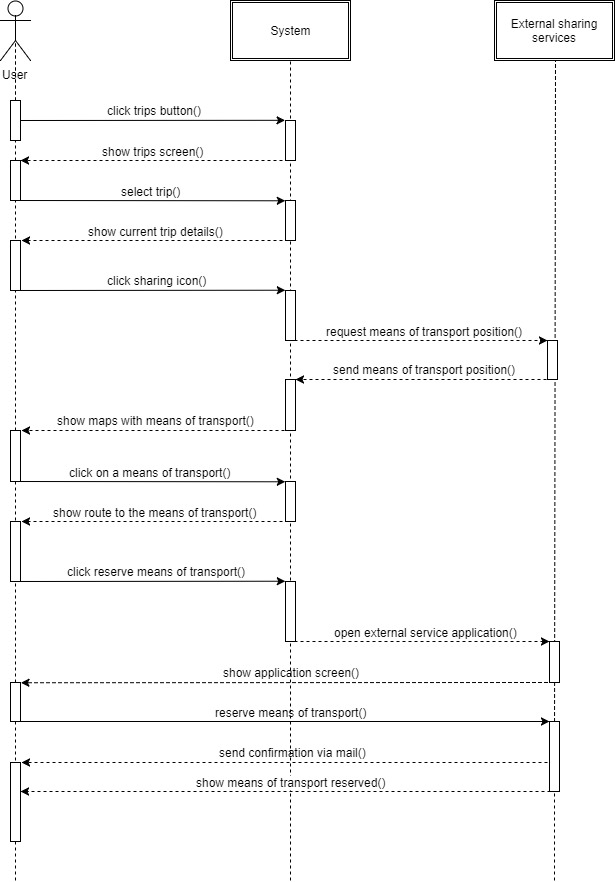
\includegraphics[scale=0.55]{MainMatter/images/sequencediagrams/reservesharing}
\captionof{figure}{Sequence diagram of reserve a sharing means of transport}
\end{center}

\begin{center}
\makebox[\textwidth][c]{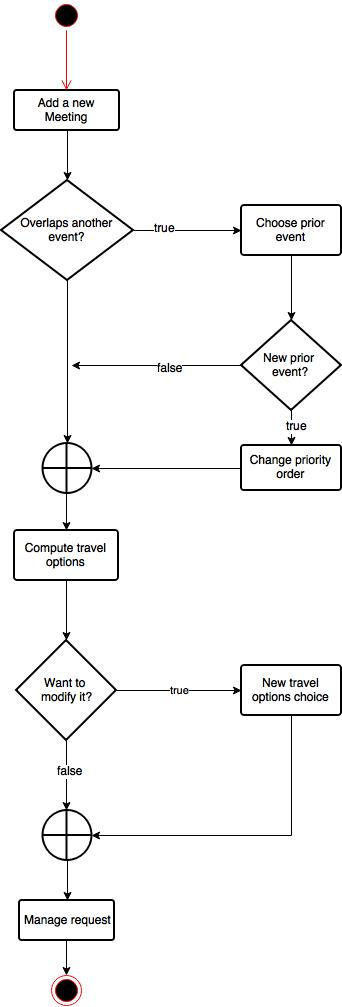
\includegraphics[width=0.485\textwidth]{MainMatter/images/activitydiagrams/addmodify}}
\captionof{figure}{System's point of view activity diagram of an event addition and trip option choice}
\end{center}
\pagebreak
%
% -----------------------------END------------------------------------- %